\chapter{METHODOLOGY}
\label{chp:methodology}

In this chapter, methodology proposed in this thesis study is presented. Firstly, approach overview is described from a high-level perspective. Then, each stage in the methodology is presented together with their importance in the study, mathematical representations and definitions; and black-box diagrams. In the last section of this chapter, implementation details of this methodology in ProM framework is explained in detail with a software architecture overview.

\section{Approach Overview}
\label{sec:approach-overview}
Approach proposed in this study consists of four main stages and general information about these stages can be summarized as following:
\begin{description}
	\item[Process Model Mining:] Process models are extracted from event logs for each organization with a user specified noise threshold.
	\item[Performance Indicator Analysis:] Event logs are replayed on process models and performance indicators are calculated for each organization. Using these indicators, organizations are clustered based on how well they are operating.
	\item[Mismatch Pattern Analysis:] Differences between process models of organization are extracted with a well-established mismatch patterns.
	\item[Recommendation Generation:] Using the performance indicator clusterings and differences between process models, a set of recommendation for each organization is generated.
\end{description}

Flow of these stages with the important input and outputs can be visualized in Figure~\ref{fig:approach-overview}. In the following sections, each stage will be explained in detail with their mathematical backgrounds.
\begin{figure}
  \centering
  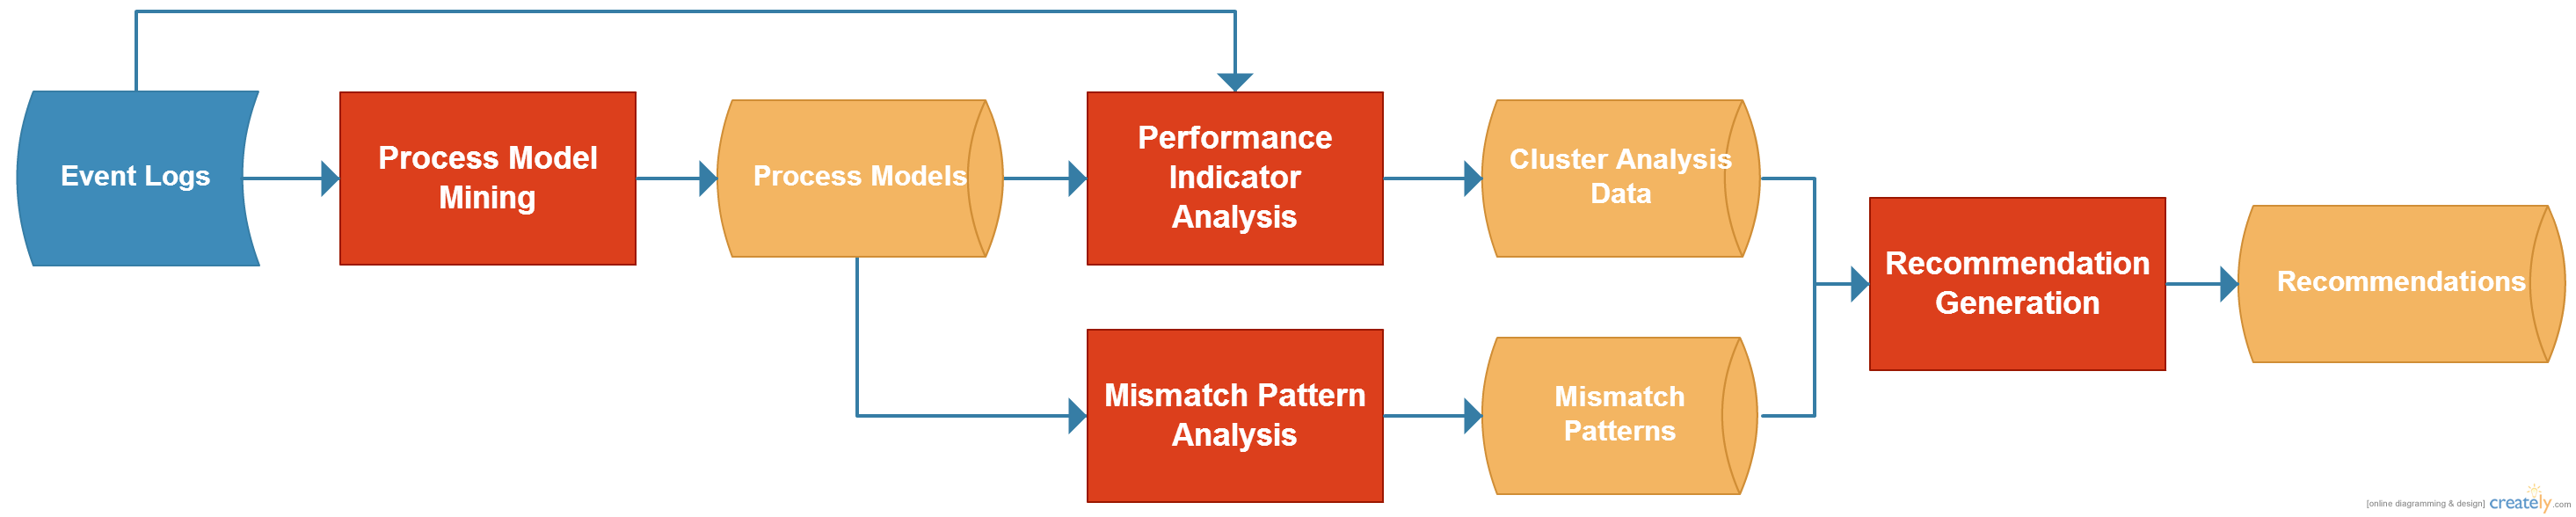
\includegraphics[width=\textwidth]{4_methodology/approach-overview}
  \caption{Overview of Methodology}
  \label{fig:approach-overview}
\end{figure}

\section{Process Model Mining}
\label{sec:process-model-mining}
Process model mining stage in the proposed approach has the aim of creating reproducible and generalized process models from event logs. In order to achieve this aim, implementation of \textit{Inductive Miner Infrequent (IMi)}, which is proposed in \cite{leemans2014discoveringinfrequent} as an extension to \textit{Inductive Miner} to handle noise in the event logs, is used in this study. 

The selected implementation has the ability of pruning data to handle noise in the event logs. Like the other data mining approaches, event logs include data related to the infrequent behaviors occurred in real life. Although these infrequent behaviors might be caused by important structural or case related issues that should be analyzed; they make the process of mining and results more complex. In the scope of this study, without cleaning the data, most of the process model mining approaches result with \textit{spaghetti-like models} \cite{van2011process} which are difficult to further analyze. Since this thesis focuses on learning from the cross-organizational process mining rather than creating the best-fitting process models, data cleaning and noise handling is a necessary step. Therefore preprocessing steps are undertaken with a compatible approach of \textit{Inductive Miner Infrequent (IMi)}, where data is cleaned in every inductive step.

Considering the scope of this study, instead of computational details of \textit{Inductive Miner Infrequent (IMi)} black-box representation is used to explain its usage in the methodology. In order to provide a filtering threshold, a user-provided value between 0 to 1 is added as input to method in addition to event logs. As a result, workflow net is produced which is a sound and properly completed Petri net without deadlocks. Black-box of this stage is illustrated in Figure~\ref{fig:process-model-mining-blackbox} and this stage is called for every organization's event logs to create their own process models in Workflow net formalization.

\begin{figure}
  \centering
  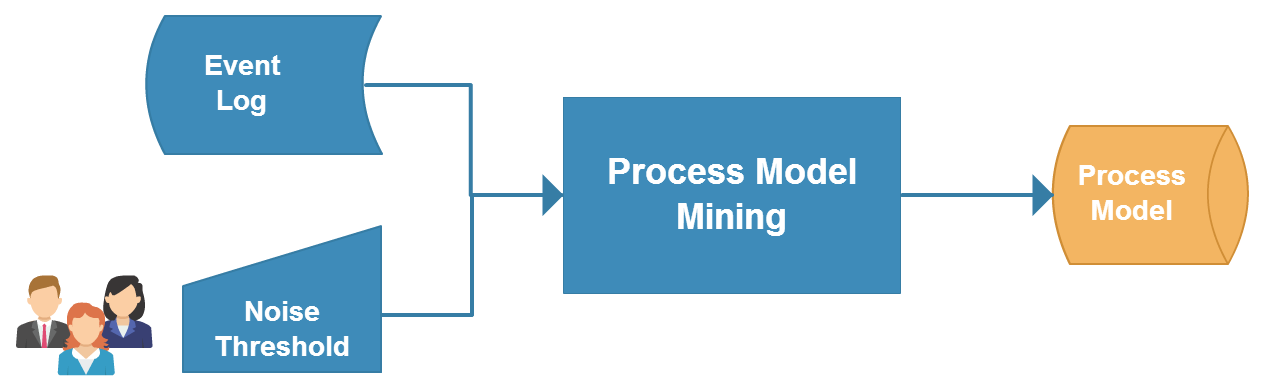
\includegraphics[width=\textwidth]{4_methodology/process-model-mining-blackbox}
  \caption{Process Model Mining Stage as Black-box }
  \label{fig:process-model-mining-blackbox}
\end{figure}


\section{Performance Indicator Analysis}
\label{sec:performance-indicator-analysis}
Performance indicator analysis stage focuses on calculating and analyzing the performance values using the event logs and mined process models. This stage consists of mainly two concepts as 
\begin{inparaenum}[\itshape a\upshape)]
\item alignment and calculation of performance indicators; and
\item clustering of organizations based on their performance values.
\end{inparaenum}
In order to evaluate the performance of an organization based on their process models and past activities; there are a number of indicators in time dimension, cost dimension and utilization \cite{van2011process}. However, in this study, process related performance values are considered since differences in the process models are studied in the next stages. With this reasoning, the following performance indicators are calculated and analyzed in this stage of methodology:
\begin{description}
  \item[Average Time Between Activities] For each activity in the process model, average time to reach other activity is calculated. This is a simple but powerful performance metric for organizations since it can yield the average time to complete one task based on a starting point. From the performance perspective, organizations want to minimize average time between activities to increase their throughput \cite{van2012replaying}. This notion can be defined as following:
	\theoremstyle{definition}
	\begin{definition}{}
	Average time between activity $A$ and $B$ in organization $i$ is 
	$AvgTime_{A\rightarrow B}^{i} = \sum_{Case\ c \in Event Log_{i}} TimeBetween_{c}(A,B) / Occurences_{Event\ Log_{i}}(A,B)$ where
		\begin{enumerate}
			\item $TimeBetween_{c}(A, B) = EndTime_{c}(B) - StartTime_{c}(A)$
			\item $StartTime_{c}(A)$ is start time of activity $A$ in case $c$,
			\item $EndTime_{c}(B)$ is end time of activity $B$ in case $c$,
			\item $Occurences_{Event Log_{i}}(A, B)$ is number of occurrences of  activity $A$ followed by $B$ in  $Event\ Log_{i}$.
		\end{enumerate}
	\end{definition}

	\item[Standard Deviation of Time Between Activities] Time between activities in real life is not stable and they deviate due to various reasons such as people responsible of tasks, size and the content of tasks or seasonality \cite{van2011process}. On the other hand, organizations want to be confident about their processes and therefore they want to minimize the deviation in the time between activities. Minimized deviation in time helps organizations to plan, act and re-organize the activities in the processes with high accuracy \cite{van2012replaying}. With the same approach above, the following formulation can be defined:
	\theoremstyle{definition}
	\begin{definition}{}
	Standard deviation time between activity $A$ and $B$ in organization $i$ is 

	$StdDevTime_{A\rightarrow B}^{i} = \sqrt{\frac{\sum_{Case\ c \in Event Log_{i}} [TimeBetween_{c}(A, B) - AvgTime_{A\rightarrow B}^{i}]^{2}}{Occurences_{Event\ Log_{i}}(A,B)} }$ 
	\end{definition}
\end{description}

In addition to average and standard deviation, minimum and maximum times between activities can also be analyzed. However, these performance values are mostly result of rare cases in the event logs and these rare occurrences have the probability of being eliminated as noise in process mining stage. Therefore, the minimum and maximum values have the risk of not representing the actual performances. Thus, only average and standard deviation of the time between activities are selected in the study. 

\subsection{Replay and Performance Indicator Calculation}
\label{subsec:replay-and-performance-summary}
Replay of event logs on process models is based on the idea of \textit{alignment} which is formalized in \cite{van2012replaying} and the basic assumption in this concept is that process models and event logs have the same activity labels. Alignment is based on \textit{moves in the model and log} and in order to have a successful replay where optimal alignment should be achieved. As proposed in \cite{adriansyah2011conformance} \cite{adriansyah2011towards}, $A^{*}$ algorithm which is a path-finding algorithm based on graphs is used to find optimal alignment of event logs on the process models.

In order to appropriately apply $A^{*}$ algorithm, there are number of manual and computational steps that should be undertaken. The following prerequisite steps are implemented in \cite{adriansyah2011towards} to apply $A^{*}$ algorithm:
 \begin{description}
	\item[Set Label Patterns between Process Model and Event Log:] In the event logs, there are various different transitions of the same activity which are generally not represented in process models. For instance, there can be \textit{"Activity A, Start"} and \textit{"Activity A, End"} in the event log; however they are reflected as \textit{"Activity A"} in the process model. Therefore, a list of all transitions and events are asked to the user to match to the ones in the process model in terms of patterns or regular expressions.
	\item[Create Initial and Final Markings:] In case of there is no definite starting or ending point in the process model, user input is necessary to define these activities.
	\item[Set Cost Values:] Since $A^{*}$ algorithm is based on alignments which are basically moves along process models and event logs, the following cost values for each move is necessary to be set:
	\begin{inparaenum}[\itshape a\upshape)]
		\item move on process model, 
		\item move on event log; and
		\item synchronous move.
	\end{inparaenum}
\end{description}
In order to use replay as an intermediate stage in this thesis, some of the mentioned steps are automatized with the help of the assumptions in the prior and post stages of methodology. With this reasoning, initial and final markings are created with the first and last activities in the process models. In addition, since there is no explicit priority of process model over event log or vice versa, cost values are set to 1 for both \textit{move on process model} and \textit{move on event log}. Since there is no penalty for \textit{synchronous moves}, their cost value is set to 0. However, since each event log has different set of transition labels, manual user input is still necessary to map label patterns between process model and event log. With the generated and user-specified inputs, replay and performance indicator calculation in the methodology can be visualized in Figure~\ref{fig:replay-and-performance-indicator-calculation}. For each organization, the steps in the diagram are followed with the corresponding event logs and process models; and the resulting process summaries are used for further analysis.

\begin{figure}
  \centering
  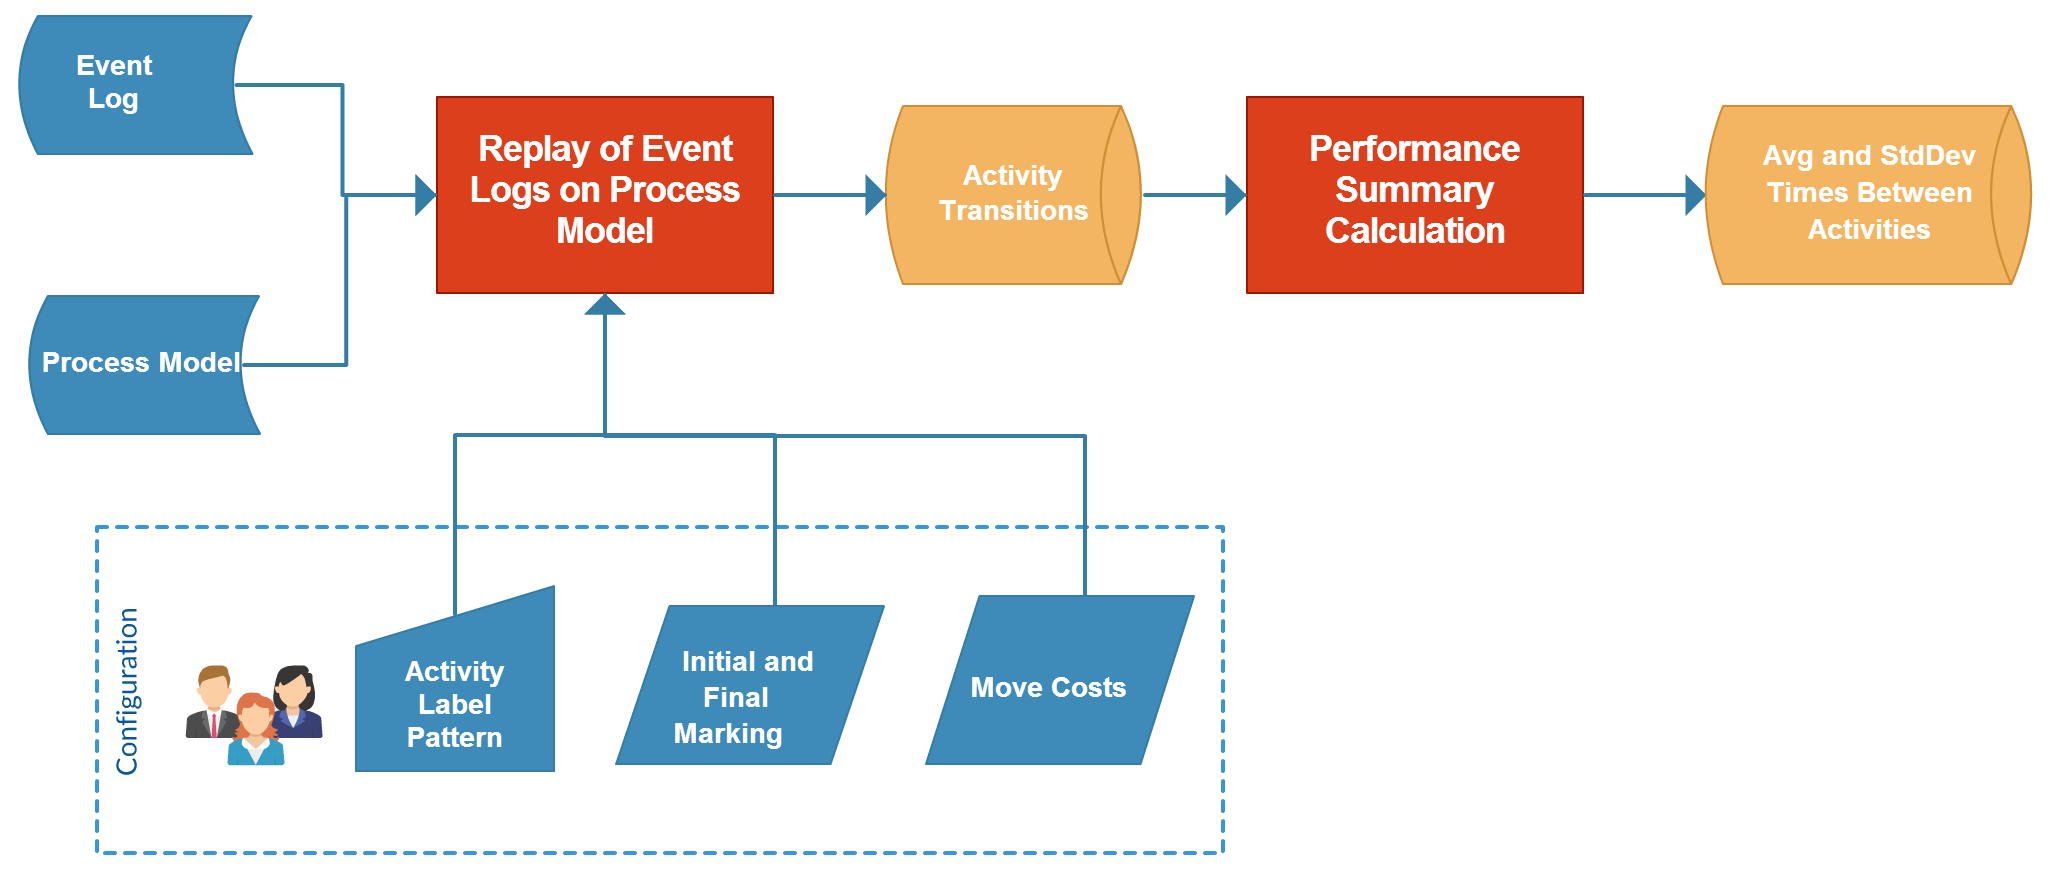
\includegraphics[width=\textwidth]{4_methodology/replay-and-performance-indicator-calculation}
  \caption{Replay and Performance Indicator Calculation Stage as Black-box}
  \label{fig:replay-and-performance-indicator-calculation}
\end{figure}

Performance summary calculation step at the end of this stage is used to create a summary of data consists of average and standard deviation of time between activities. Resulting data can be defined as following:
	\theoremstyle{definition}
	\begin{definition}{} Performance Summary data for any organization $i$ is 

	$PerfSum_{i}= \{AvgTimeSum_{i}\ \cup\ StdDevTimeSum_{i}\}$ where
		\begin{enumerate}
			\item $AvgTimeSum_{i} = \{ AvgTime_{A \rightarrow B}^{i} | A , B  \in Event\ Log_{i}\}$
			\item $StdDevTimeSum_{i} = \{ StdDevTime_{ A\rightarrow B}^{i} | A, B  \in Event\ Log_{i}\}$
		\end{enumerate}
	\end{definition}

\subsection{Performance Indicator Clustering}
\label{subsec:performance-indicator-clustering}

Clustering is based on the idea of collecting the set of observations into clusters so that observations within the same cluster are similar whereas the observations from different clusters are dissimilar. Being a unsupervised learning method, it aims to find hidden structures in unlabeled data. In this thesis study, clustering is used to cluster organizations based on their performance indicator data. In other words, organizations will be set into groups based on how much time in average and with variation takes to complete an activity given a starting point.

Within clustering analysis, various algorithms are proposed to find clusters based on the idea of decreasing in-cluster distances, increasing space density or fitting to particular statistical distributions. However, in this study, a generic approach based on centroid-based clustering is exploited. For the fixed number of \textit{k} clusters, the approach is well-known as \textit{k-means clustering}. Considering the popularity of this approach and its extensions, random initialization based \textit{k-means++} approach from the study of Arthur and Vassilvitskii \cite{arthur2007} is used to cluster organizations. 

Clustering methods can be evaluated by the internal and external methods. Internal methods are based on the data that is clustered itself whereas external methods use the additional information such as labels or benchmarks. Although there are various well-established metrics in external methods such as Rand Measure, F-measure, Jaccard index or Confusion Matrices; in this thesis study there is no pre-labeled organizations based on their performance indicators. Therefore, internal evaluation methods are used to assess the quality of clusters. Considering the fact that actual data to cluster is \textit{time interval} and centroid-based clustering is applied in this study, a metric based on decreasing the in-cluster distances is selected. With this consideration, Sum of Squared Error (SSE) is calculated with the following definition. When the clustering results are compared, it is reasonable to choose the one with the least SSE; however, it is a fact that as \textit{k} converges to the number of original sample size SSE value decreases. Therefore, SSE values and number of clusters are plotted and presented to the end user of the methodology to select optimal number of clusters.

\theoremstyle{definition}
\begin{definition}
Sum of Squared Error (SSE) is

$SSE = \sum_{i=1}^{k} \sum_{x \in c_{i}} EuclideanDistance(mean_{i}, x)^{2}$ where
\begin{enumerate}
  \item $x$ is a data point in cluster $c_{i}$.
  \item $mean_{i}$ is the mean vector of the cluster $c_{i}$.
\end{enumerate}
\end{definition}

For each organization, \textit{Performance Summary} data is used as the data source in clustering. It is aimed that the organizations with the similar average or standard deviation time between tasks will be assigned to same sets to further reveal the dissimilarities that the other clusters can learn from. Since not every activity exists in every organization, performance summary data is cleaned and merged to include only all shared activities. This cleaning step removes the non-existing activity related performance indicators from all the organizations so that clustering is applied on the data with no process model related information. Since number of clusters are not known priori, k-means clustering is applied starting \textit{k} from 1 to the number of organizations. For each clustering with different number of clusters, SSE values are plotted and user is made to select the appropriate cluster size. For the selected cluster size, clustering related information is used to generate recommendations in the further steps. This stage of methodology can be visualized as an input-output system in Figure~\ref{fig:performance-indicator-clustering-blackbox}. Resulting cluster analysis data is formulated as following:

\theoremstyle{definition}
\begin{definition}
Cluster Analysis Data is a tuple $(k, Assignments, Cluster\ Centroids)$ where
\begin{enumerate}
	\item $k$ is the number of clusters,
	\item $Assignments$ is a set of tuple $(Organization_{i}, Cluster_{j})$ where $i$ is identifier for organization and $j \leq k$ is identifier for cluster,
	\item $Cluster\ Centroids$ is a set of tuple $(Cluster_{j}, Type, A_{start}, A_{end}, Value)$ where
		\begin{enumerate}
			\item $Type$ is performance indicator type which is $Average$ or $StandardDev$,
			\item $A_{start}$ and $A_{end}$ are starting and ending points of performance indicator,
			\item $Value$ is the actual value of performance indicator,
			\item $Cluster\ Centroids_{j}$ is a function that returns set of $Centroid$ which are tuples of $(Type, A_{start}, A_{end}, Value)$ for $Cluster_{j}$.
		\end{enumerate}	
\end{enumerate}
\end{definition}
 
\begin{figure}
  \centering
  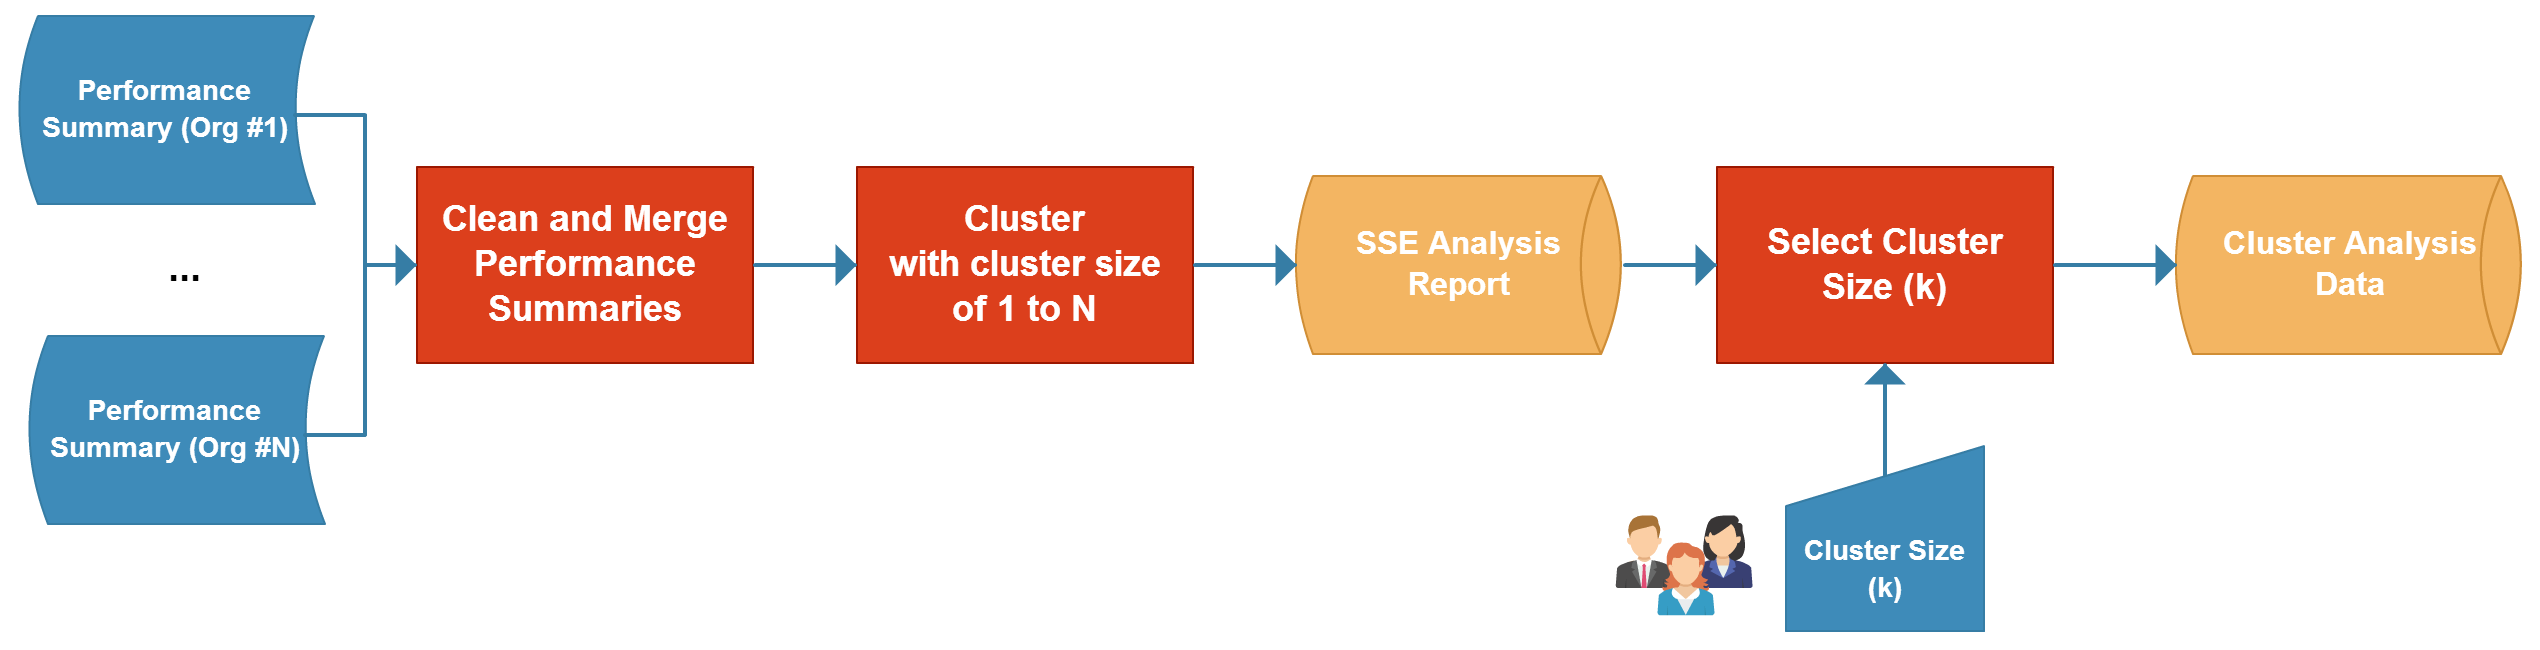
\includegraphics[width=\textwidth]{4_methodology/performance-indicator-clustering-blackbox}
  \caption{Performance Indicator Clustering Stage as Black-box }
  \label{fig:performance-indicator-clustering-blackbox}
\end{figure}
 
\section{Mismatch Pattern Analysis}
\label{sec:mismatch-pattern-analysis}
In order to learn from other organizations, it is necessary to spot the differences between process models of different organizations. In this phase of methodology, differences between process models will be revealed by the mismatch patterns which are defined by Dijkman \cite{dijkman2007mismatch}. In the process mining stage, process models are mined to create Workflow nets; however, mismatch pattern definitions are closer to business environment and it is more suitable spot patterns in BPMN notation. Thus, mined process models are converted to BPMN models and then mismatch pattern analysis is applied. After spotting differences, mismatch patterns for activities and control flows average revealed for the organizations.

Business Process Modeling Notation (BPMN) is one of the widely accepted modeling language in the industry and its a standardized notation by the Object Management Group (OMG) since 2004. Main aim of BPMN is to provide a notation that is easily understood by business stakeholders. In the preceding stages, Petri nets and their subset as Workflow nets are used for mining since they have stronger mathematical background. However, in this stage, BPMN formulation is used since mismatch patterns have roots in real-life business environment \cite{dijkman2007mismatch}. The following definition and conversion are defined in the study \cite{kalenkovaprocess} and they are used in the mismatch pattern analysis. 

\theoremstyle{definition}
\begin{definition}
A BPMN model is a tuple 

$BPMN_{model}=(N, A, G_{XOR}, G_{AND}, e_{start}, E_{end}, SF, \lambda)$ where
\begin{enumerate}
  \item $N$ is a set of flow nodes,
  \item $A \subseteq N$ is a set of activities,
  \item $G_{XOR} \subseteq N$, $G_{AND} \subseteq N$ are sets of exclusive and parallel gateways,
  \item $e_{start} \in N$ is a start event,
  \item $E_{end} \in N$ is a set of end events,
  \item Sets $A, G_{XOR}, G_{AND}, \{e_{start}\}, E_{end}$ form a partition of N,
  \item $SF \subseteq N \times N$ is a set of sequence flows,
  \item $\lambda : N \rightarrow U_{A}$ is a labeling function, where $U_{A}$ is some universe of activity labels,
  \item Start event $e_{start}$ does not have incoming sequence flows and has not more than one outgoing sequence flows,
  \item End events $E_{end}$ do not have outgoing sequence flows.  
\end{enumerate}
\end{definition}

\theoremstyle{definition}
\begin{definition}
Constructing BPMN Model from Petri nets, which are $N = (P, T, F)$ where $P$ is finite set of \textit{places}, $T$ is finite set of \textit{transitions} and $F$ is set of \textit{flow relations} to BPMN models consists of the following steps:
\begin{enumerate}
  \item Initialize BPMN model with a start node $e_{start}$.
  \item Convert all transitions, $T$, in the Petri net by creating an activity in BPMN model for each transition in Petri net.
  \item Convert all places, $P$, from Petri net to BPMN routing constructs by finding the corresponding sequence flows.
\end{enumerate}
\end{definition}

For each organization, mined process models are converted to BPMN models and mismatch patterns analysis is undertaken on them. For each mismatch pattern analysis, the aim is to locate differences between two process models or cluster of process models. In addition, since performance indicators are calculated based on a starting and ending point in the process model, same approach is applied to locate mismatch patterns. In other words, differences of process models are located through a starting activity to an ending activity. This approach also enables to locate the whole set of mismatches between process models when starting and ending points are provided as source and sink activities. Mismatch patterns are formulated and their importance in the methodology are listed as following:
\begin{description}
  \item[Skipped Activity] Skipped activities are the operations that are not undertaken with some of the organizations. In business environment there could be various different reasons for an organization to exclude any activity in their process flows which are followed by other organizations. Therefore, this mismatch pattern should not be utilized solely but taken in to care with the other patterns. In this study, for each organization a list of activities that they do not include are listed as \textit{Skipped Activity} with the following definition. In addition, these differences are checked for the activities with a particular start and end point. 
		\theoremstyle{definition}
		\begin{definition}
		Skipped Activity pattern is a tuple 

		${Skipped\ Activity} = (O, SA, A_{start}, A_{end}) $ where 
		\begin{enumerate}
		  \item $O$ is the identifier for organization,
		  \item BPMN model of organization is $BPMN_{O}$ and $BPMN_{*}$ is the set of all BPMN models in analysis,
		  \item $SA$ is a set of skipped activities and $SA =  BPMN_{*}(A) \setminus BPMN_{O}(A)$,
		  \item $A_{start}$ and $A_{end}$ are starting and ending points to check mismatch patterns and $A_{start}, A_{end} \in BPMN_{O}(A)$.
		\end{enumerate}
		\end{definition}

		\theoremstyle{definition}
		\begin{definition}
		Skipped Activity Analyzer is a function 

		$SkippedActivityAnalyzer(O, A_{start}, A_{end})$ and it returns a set of \textit{Skipped Activity} for the organization $O$ and the activities between $A_{start}$ and $A_{end}$.
		\end{definition}
  \item[Refined Activity] Refined activities exist in one process; however, as equivalent a collection of activities are undertaken in another organization's process to achieve the same task. Since there is no activity ontology information is kept in event logs and process models, there is no direct method to define whether the tasks can be classified as other tasks' refined state. In this study, assuming the labels of activities are correct and explanatory about their enclosures, similarity between labels are utilized for this aim. Using \textit{Levenshtein distance}, which is very popular in information retrieval area and also known as \textit{edit distance}, similarity of activity labels are calculated for each activity in respect to activities of other organizations' process models. This mismatch pattern presents information about the similar but not same activities in different process models which can be used to make organizations learn from each other. With a user-defined threshold for similarity based on the nature of business environment, most similar tasks can be listed for being refined.
		\theoremstyle{definition}
		\begin{definition}
		Refined Activity pattern is a tuple 

		${Refined\ Activity} = (O_{1}, O_{2}, RA, SimilarityMap, A_{start}, A_{end}) $ where 
		\begin{enumerate}
		  \item $O_{1}$ is the first organization where the refined activity is undertaken with the BPMN model of $BPMN_{{O}_{1}}$,
		  \item $O_{2}$ is the second organization where a collection of activities checked for similarity with the BPMN model of $BPMN_{{O}_{2}}$,
		  \item $RA$ is the refined activity and $RA \in BPMN_{{O}_{1}}(A)$ and $RA \notin BPMN_{{O}_{2}}(A)$,
		  \item $SimilarityMap$ is a set of tuples $(SimilarityValue, A)$ where $SimilarityValue$ indicates the similarity between $RA$ and $A \in BPMN_{{O}_{1}}(A)$, 
 		  \item $A_{start}$ and $A_{end}$ are starting and ending points to check mismatch patterns and $A_{start}, A_{end} \in BPMN_{{O}_{1,2}}(A)$. 
		\end{enumerate}
		\end{definition}

		\theoremstyle{definition}
		\begin{definition}
		Refined Activity Analyzer is a function 

		$RefinedActivityAnalyzer(O_{1}, O_{2}, A_{start}, A_{end})$ and it returns a set of \textit{Refined Activity} for the organization $O_{1}$ compared to $O_{2}$ for the activities between $A_{start}$ and $A_{end}$.
		\end{definition}

   \item[Activities at Different Moments in Processes] Activities at different moments means that organizations are undertaking activities at different orders in their process flows. This mismatch pattern indicates that the organizations could achieve the same task when they change the order of activities and this information can be used by others to enhance their process models. Therefore, formulation of this pattern includes an activity; and its previous and next tasks at different organizations.
		\theoremstyle{definition}
		\begin{definition}
		Activities at Different Moments in Processes pattern is a tuple 

		${Different\ Moments} = (O_{1}, O_{2}, A, Prev_{1}, Next_{1},Prev_{2}, Next_{2}, A_{start}, A_{end}) $ where 
		\begin{enumerate}
		  \item $O_{1}$ is the first organization with the BPMN model of $BPMN_{{O}_{1}}$,
		  \item $O_{2}$ is the second organization with the BPMN model of $BPMN_{{O}_{2}}$,
		  \item $A$ is the activity that is undertaken in different order and $A \in BPMN_{{O}_{1,2}}(A)$,
		  \item $Prev_{1}, Next_{1},$ are previous and next tasks of $A$ in $O_{1}$ and  $Prev_{1}, Next_{1} \in  BPMN_{{O}_{1}}(A)$,
  		  \item $Prev_{2}, Next_{2},$ are previous and next tasks of $A$ in $O_{2}$ and  $Prev_{2}, Next_{2} \in  BPMN_{{O}_{2}}(A)$,
  		  \item In order to ensure different moments $Prev_{1} \neq Prev_{2}$ or $Next_{1} \neq Next_{2}$,
 		  \item $A_{start}$ and $A_{end}$ are starting and ending points to check mismatch patterns and $A_{start}, A_{end} \in BPMN_{{O}_{1,2}}(A)$. 
		\end{enumerate}
		\end{definition}

		\theoremstyle{definition}
		\begin{definition}
		Different Moments Analyzer is a function 

		$DifferentMomentsAnalyzer(O_{1}, O_{2}, A_{start}, A_{end})$ and it returns a set of \textit{Different Moments} for the organization $O_{1}$ compared to $O_{2}$ for the activities between $A_{start}$ and $A_{end}$.
		\end{definition}

	\item[Different Conditions for Occurrence] Different conditions for occurrence take place where an activity has the same dependencies in different organizations but with different conditions. For instance, an organization needs to complete all dependency tasks before starting the next one; though another organization checks for the completion of only one of these dependencies. This difference between organizations can lead to loosen or tighten the conditions based on the application of other organizations. Considering the representation of different conditions for occurrence and other control flow mismatch patterns, a generic definition is developed firstly to use and further customize. Different conditions for occurrence pattern definition is developed based on this generic definition as following.
		\theoremstyle{definition}
		\begin{definition}
		Control Flow Mismatch pattern is a tuple 

		${Control\ Flow\ Mismatch} = (O_{1}, O_{2}, A, Prev_{1}, G_{1}, Prev_{2}, G_{2}, A_{start}, A_{end}) $ where 
		\begin{enumerate}
		  \item $O_{1}$ is the first organization with the BPMN model of $BPMN_{{O}_{1}}$,
		  \item $O_{2}$ is the second organization with the BPMN model of $BPMN_{{O}_{2}}$,
		  \item $A$ is the activity that is in front of control flow and $A \in BPMN_{{O}_{1,2}}(A)$,
		  \item $Prev_{1}$ and $Prev_{2}$ are set of tasks that are connected to gateway $G_{1}$ and $G_{2}$ in organizations $O_{1}$ and $O_{2}$ respectively with the following requirements:
			  \begin{enumerate}
				  \item $Prev_{1} \subset BPMN_{{O}_{1}}(A)$,
				  \item $Prev_{2} \subset BPMN_{{O}_{2}}(A)$,
				  \item $G_{1} \in BPMN_{{O}_{1}}(G_{XOR}, G_{AND})$,
	  			  \item $G_{2} \in BPMN_{{O}_{2}}(G_{XOR}, G_{AND})$.
			  \end {enumerate}
 		  \item $A_{start}$ and $A_{end}$ are starting and ending points to check mismatch patterns and $A_{start}, A_{end} \in BPMN_{{O}_{1,2}}(A)$. 
		\end{enumerate}
		\end{definition}

		\theoremstyle{definition}
		\begin{definition}
		Different Conditions for Occurrence pattern is a \textit{Control Flow Mismatch} where
		\begin{enumerate}
			\item $Prev_{1} = Prev_{2}$,
			\item $G_{1} \neq G_{2}$.
		\end{enumerate}
		\end{definition}

		\theoremstyle{definition}
		\begin{definition}
		Different Conditions Analyzer is a function 

		$DifferentConditionsAnalyzer(O_{1}, O_{2}, A_{start}, A_{end})$ and it returns a set of \textit{Different Conditions for Occurrence} for the organization $O_{1}$ compared to $O_{2}$ for the activities between $A_{start}$ and $A_{end}$.
		\end{definition}	

	\item[Different Dependencies] When the dependency set of a specific activity is different in organizations, it can be concluded that this activity and the relation between its dependency sets should be reviewed since it can be achieved in both environments. Organizations can learn from each other to eliminate or enhance their process flows by changing these dependency sets. This can include re-organization of activities as well as removing and adding new activities. The idea is structured in the following simplified definition.
		\theoremstyle{definition}
		\begin{definition}
		Different Dependencies pattern is a \textit{Control Flow Mismatch} where
		\begin{enumerate}
			\item $Prev_{1} \neq Prev_{2}$,
			\item $G_{1} = G_{2}$.
		\end{enumerate}
		\end{definition}

		\theoremstyle{definition}
		\begin{definition}
		Different Dependency Analyzer is a function 

		$DifferentDependencysAnalyzer(O_{1}, O_{2}, A_{start}, A_{end})$ and it returns a set of \textit{Different Dependency} for the organization $O_{1}$ compared to $O_{2}$ for the activities between $A_{start}$ and $A_{end}$.
		\end{definition}	
	\item[Additional Dependencies] Additional dependency pattern is a special case of \textit{Different Dependencies} where additional tasks are required in one organization in order to start an activity. These additional dependencies can include provisional tasks that are related to the original activity such as \textit{checking system} before \textit{starting application}. 
		\theoremstyle{definition}
		\begin{definition}
		Additional Dependencies pattern is a \textit{Different Dependencies Mismatch} where $Prev_{1} \subseteq Prev_{2}$ or $Prev_{1} \subseteq Prev_{2}$.
		\end{definition}

		\begin{definition}
		Additional Dependency Analyzer is a function 

		$AdditionalDependencysAnalyzer(O_{1}, O_{2}, A_{start}, A_{end})$ and it returns a set of \textit{Additional Dependency} for the organization $O_{1}$ compared to $O_{2}$ for the activities between $A_{start}$ and $A_{end}$.
		\end{definition}	
 \end{description}
 
Mismatch pattern analysis stage in methodology can be visualized as a black-box diagram in Figure\ref{fig:mismatch-pattern-analysis-blackbox}. Each organization's mined process models are converted to BPMN models and these models are sent so mismatch pattern analyzers with the starting and ending activities. For each organization, mismatch patterns are gathered and stored for the further analysis as presented in Algorithm~\ref{algo:mismatch}.
\begin{figure}
  \centering
  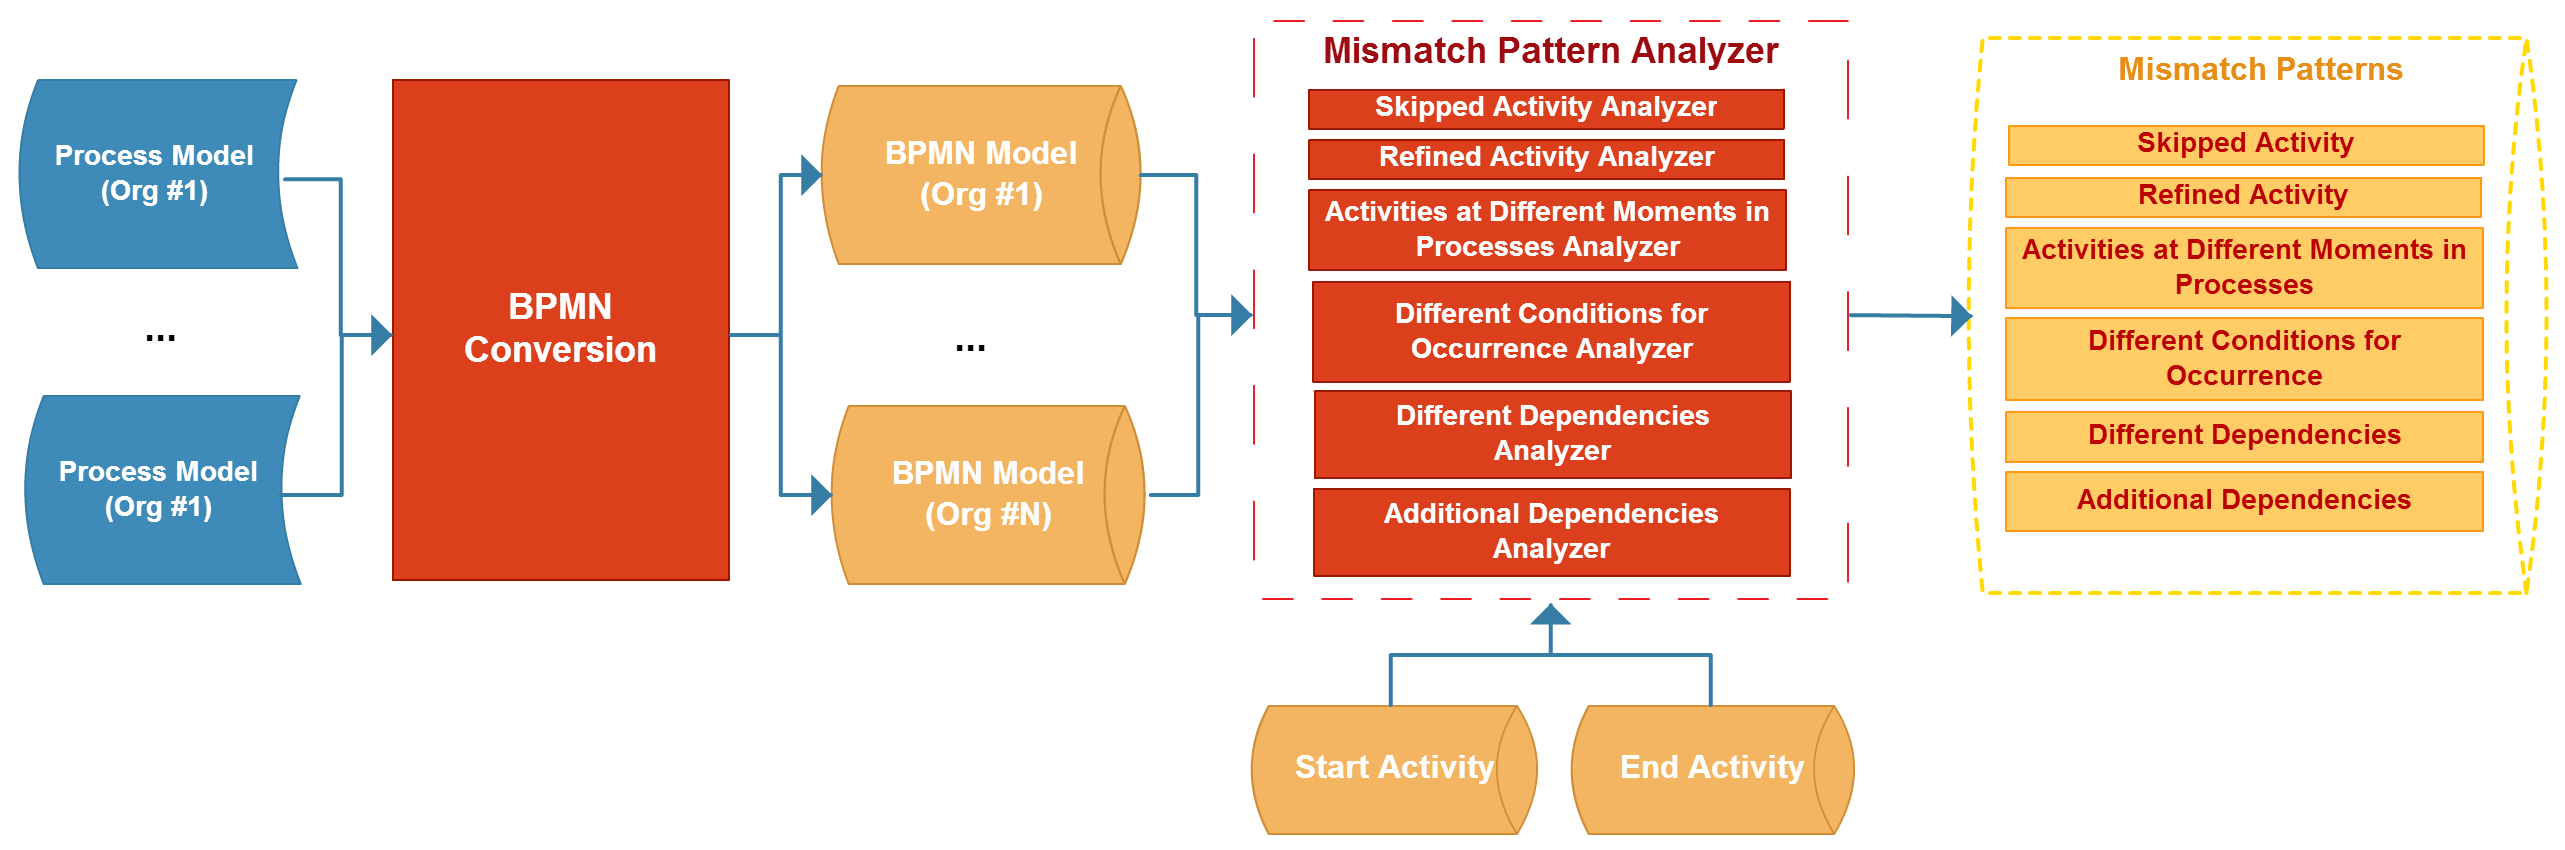
\includegraphics[width=\textwidth]{4_methodology/mismatch-pattern-analysis-blackbox}
  \caption{Mismatch Pattern Analysis Stage as Black-box}
  \label{fig:mismatch-pattern-analysis-blackbox}
\end{figure}

\begin{algorithm}
\DontPrintSemicolon % Some LaTeX compilers require you to use \dontprintsemicolon instead 
\KwIn{$O_{1}$ first organization, $O_{2}$ second organization, $A_{start}$ starting activity, $A_{end}$ ending activity}
\KwOut{$MismatchPatterns$ a set of mismatch patterns}
$MismatchPatterns \leftarrow \{\}$ \;
$MismatchPatterns$ \leftarrow  SkippedActivityAnalyzer($O_{1}$,$A_{start}$,$A_{end}$) \;
$MismatchPatterns$ \leftarrow  RefinedActivityAnalyzer($O_{1}$,$O_{2}$,$A_{start}$,$A_{end}$) \;
$MismatchPatterns$ \leftarrow  DifferentMomentsAnalyzer($O_{1}$,$O_{2}$,$A_{start}$,$A_{end}$) \;
$MismatchPatterns$ \leftarrow  DifferentConditionsAnalyzer($O_{1}$,$O_{2}$,$A_{start}$,$A_{end}$) \;
$MismatchPatterns$ \leftarrow  DifferentDependencysAnalyzer($O_{1}$,$O_{2}$,$A_{start}$,$A_{end}$) \;
$MismatchPatterns$ \leftarrow  AdditionalDependencysAnalyzer($O_{1}$,$O_{2}$,$A_{start}$,$A_{end}$) \;
\Return{$MismatchPatterns$}\;
\caption{Mismatch Pattern Analysis}
\label{algo:mismatch}
\end{algorithm}

\section{Recommendation Generation}
\label{sec:recommendation-generation}
Recommendation generation stage in the methodology is the final and core stage where all information retrieved from event logs until now are utilized. Till this point, all event logs are used to mine process models of each organization and then these event logs are replayed on the process models to calculate performance indicators. Following these steps, the organizations are clustered based on their performance indicators and mismatches between their process models are listed. In this stage, clustering results, which are performance indicator vectors for each cluster will be used to generate recommendations for each cluster of organizations based on the differences between their mismatch patterns.

In this study, idea of recommendation is based on providing a set of mismatch patterns for each organization so that they can enhance their processes. These mismatch patterns are generated by comparing the process models of other organizations, particularly which are performing better in terms of their performance indicator values. In addition, clustering of organizations is undertaken generalize the way of identifying which organizations perform better in this environment. Recommendation idea and recommendation generation function is defined as following:
\theoremstyle{definition}
\begin{definition}
Recommendation is a tuple 

${Recommendation} = (O, A_{start}, A_{end}, Mismatch\ Patterns) $ where 
	\begin{enumerate}
	  \item $O$ is identifier for organization,
	  \item $A_{start}$ and $A_{end}$ are starting and ending activities in between the recommendations are checked,
	  \item $Mismatch\ Patterns$ is collection of mismatch patterns.
	\end{enumerate}
\end{definition}

\theoremstyle{definition}
\begin{definition}
Recommendation generation is a function that is \textit{RecGen(O, C, P)} and it returns a set of \textit{Recommendation} where
	\begin{enumerate}
	  \item $O$ is identifier for organization,
	  \item $C$ is \textit{Cluster Analysis Data} which is result of cluster analysis stage,
	  \item $P$ is \textit{Performance Threshold} which is a real number larger than or equal to 0.
	\end{enumerate}
\end{definition}

Algorithm of recommendation generation function is based on the idea of checking other clusters for a significant change in performance indicators, where significance is defined by the threshold provided by user. After finding significant difference, all organizations in other clusters are checked against mismatch patterns with the starting and ending activities defined in performance indicators. With this constraining, only mismatches which are located between the activities that causes high level of difference in performance indicators are analyzed. This approach is formalized in Algorithm~\ref{algo:recgen}.
 \begin{algorithm}
\DontPrintSemicolon % Some LaTeX compilers require you to use \dontprintsemicolon instead 
\KwIn{$O$ organization, $C$ Cluster Analysis Data, $P$ performance difference threshold}
\KwOut{$Recommendations$ a set of recommendations}
$Recommendations \leftarrow \{\}$ \;
$i \leftarrow C(Assignments(O))$ \;
\For{$Centroid \in C(Cluster Centroids_{i})$} { 
	\For{$Centroid' \in C(Cluster Centroids_{j}))\ i\neq j$} { 
		\If{$Centroid(A_{start}) = Centroid'(A_{start}) \& Centroid(A_{end}) = Centroid'(A_{end})$} {
			\If{ ($\left |  Centroid(Value) -  Centroid'(Value)\right | \div Centroid(Value)) \geq P$  } {
				$A_{start} \leftarrow Centroid(A_{start})$ \;
				$A_{end} \leftarrow Centroid(A_{end})$ \;
				$MismatchPatterns \leftarrow \{\}$ \;
		 		\For{$O' \in C(Assignments(j))$} {
					$MismatchPatterns$ \leftarrow  Mismatch Pattern Analysis($O$,$O'$,$A_{start}$,$A_{end}$) \;
				}
				$Recommendations$ \leftarrow  Recommendation($O$,$A_{start}$,$A_{end}$, $MismatchPatterns$) \;
			}
		}
	}
}
\Return{$Recommendations$} \;
\caption{Recommendation Generation}
\label{algo:recgen}
\end{algorithm}

This stage of methodology can be visualized as gathering inputs of mismatch patterns data and cluster analysis data in Figure~\ref{fig:recommendation-generation-blackox}. In addition, a performance difference threshold is gathered from the user to specify how much difference between clusters is necessary to check for mismatch patterns and generate recommendations. This stage generates recommendation data for each organization which contains a set of mismatch patterns.
\begin{figure}
  \centering
  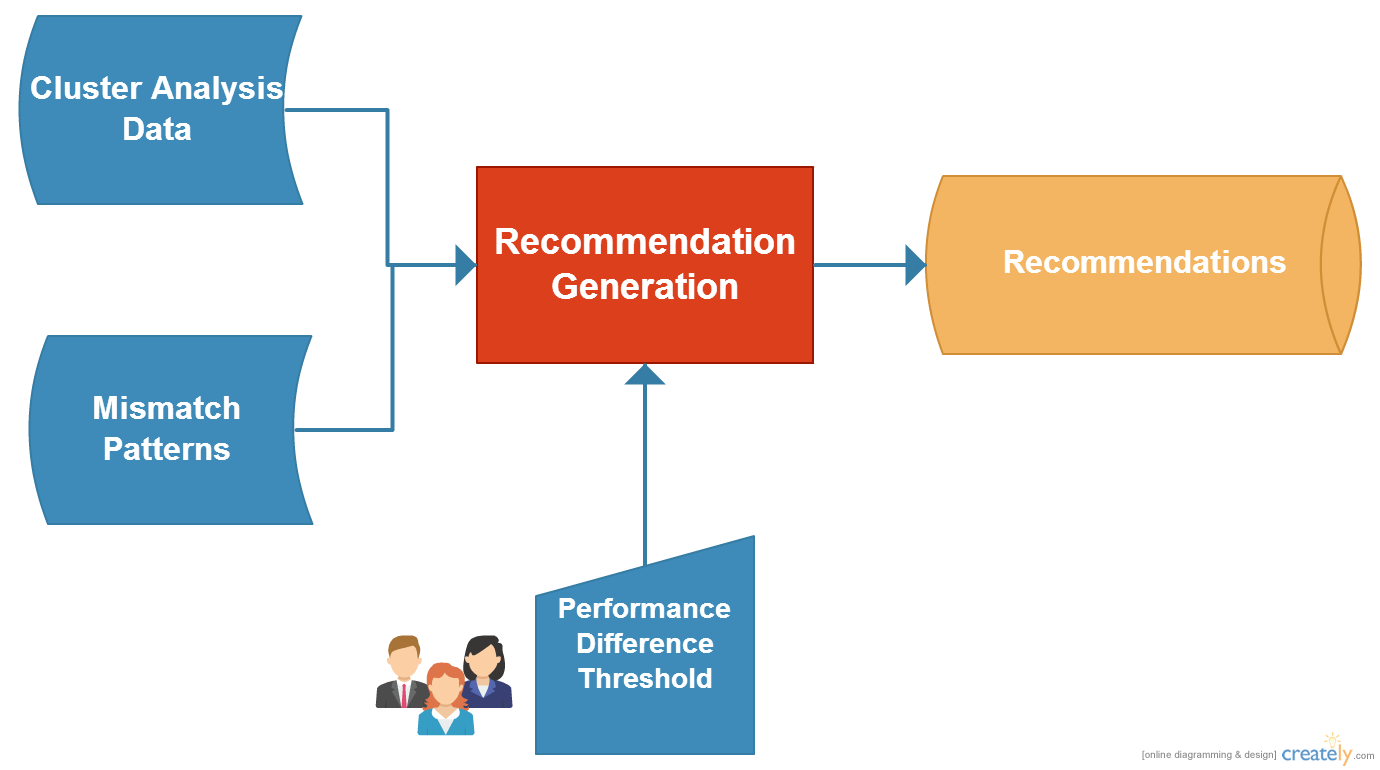
\includegraphics[width=\textwidth]{4_methodology/recommendation-generation-blackbox}
  \caption{Recommendation Generation Stage as Black-box}
  \label{fig:recommendation-generation-blackox}
\end{figure}

\section{Implementation in ProM Framework}
\label{sec:implementation}
\todo{WRITE}

Methodology of this thesis study is implemented in ProM Framework \cite{verbeek2010prom}, which is an extensible framework that supports a wide variety of process mining techniques in the form of plugins. Approach of this thesis study is implemented with its each stage as a standalone plugin that enables extensions for further studies. Developed set of plugins are packaged with the name of \textit{CrossOrgProcMin} and it is available in the latest version of ProM release. 

PROM öv

Implementation details are presented from two perspectives in this section. Firstly, software architecture of methodology implementation will be explained with the relationships and dependencies with other plug-ins and ProM framework. Then, user experience perspective will be presented to show how an end user of this methodology can provide inputs, make analysis and gather results. 

\subsection{Software Architecture}
\label{subsec:architecture}
Approach of this study is divided into standalone stages where inputs and outputs between them are defined strictly. With the help of this understanding, each stage is developed as a standalone plugin in ProM framework which can be called separately. For this aim, five plugins are developed which are visualized in Fig~XX to provide a high-level perspective. In addition, a set of utilities are developed to visualize and persistence of data in ProM environment. 

\begin{description}
  \item[Cross-Organizational Process Mining] is the core plugin which handles management and data flow between other plugins. It basically calls each other plugin and gathers outputs from them to proceed to next plugins. 
  \item[Process Miner Plugin] is the implementation of Section~\ref{sec:process-model-mining} where \textit{Inductive Miner} \cite{leemans2014discoveringinfrequent} package in the ProM environment is utilized. 
  \item[Automated Replayer Plugin] is developed to execute the approach in Section~\ref{subsec:replay-and-performance-summary} and it replays the event logs over process models with the minimum manual user input using the libraries in \textit{Peti Net Replayer} package \cite{adriansyah2011towards}. 
  \item[Cluster Analysis Plugin] is developed to cluster the organizations based on their performance indicators as presented in Section~\ref{subsec:performance-indicator-clustering} and this plugin uses WEKA libraries \cite{hall2009} which are external to the ProM environment. 
  \item[Mismatch Analysis Plugin] is developed to discover differences between the process models as explained in Section~\ref{sec:mismatch-pattern-analysis}. This plugin is developed from scratch since there is no implementation of mismatch patterns \cite{dijkman2007mismatch} in ProM framework.
  \item[Utilities] are developed to handle input and output data to the developed set of plugins. Import and export libraries are coded to enable data specific persistence in ProM framework for these plugins. Visualization libraries are developed to represent the recommendation output to the end user in ProM screens.
\end{description}   


\subsection{User Experience}
\label{subsec:architecture}
toplama olduğunu, user için gerekenleri bahset

